\documentclass{ximera}
\usepackage{../OERLinearAlgebra}

\usepackage{mathtools}

\author{Anna Davis \and Paul Zachlin \and Rosemarie Emanuele} \title{Introduction to Systems of Linear Equations} \license{CC-BY 4.0}

\begin{document}

\begin{abstract}
 We solve systems of equations in two and three variables and interpret the results geometrically.
\end{abstract}
\maketitle

You have certainly studied linear equations for many years now.  Perhaps the easiest way to characterize linear equations is that they are polynomial equations where each term is either a constant or has degree 1.

\begin{definition}
A linear equation in variables $x_1, \ldots, x_n$ is an equation that can be written in the form
$$a_1x_1+a_2x_2+\ldots +a_nx_n=b$$
where $a_1,\ldots ,a_n$ and $b$ are constants.
\end{definition}



% An $n$-tuple $(x_1, x_2,\ldots ,x_n)$ is a \dfn{solution} to the equation $a_1x_1+a_2x_2+\ldots +a_nx_n=b$ provided that it turns the equation into a true statement.  The set of all $n$-tuples that are solutions to a given equation is called the \dfn{graph} of the equation. The graph of a linear equation in two variables is a line in $\RR^2$.  The graph of a linear equation in three variables is a plane in $\RR^3$.

An $n$-tuple $(x_1, x_2,\ldots ,x_n)$ is a \dfn{solution} to the equation $a_1x_1+a_2x_2+\ldots +a_nx_n=b$ provided that it turns the equation into a true statement.  The set of all $n$-tuples that are solutions to a given equation is called the \dfn{graph} of the equation. The graph of a linear equation in two variables is a line in $\RR^2$.  The graph of a linear equation in three variables is a plane in $\RR^3$.  In $\RR^n$ for $n>3$, we say that the graph of a linear equation is a \dfn{hyperplane}. A hyperplane cannot be visualized, but we can still talk about intersections of hyperplanes and their other attributes in algebraic terms.  

In linear algebra, we often look for solutions to \dfn{systems of linear equations} or \dfn{linear systems}.  
A linear system of $m$ equations and $n$ unknowns is typically written as follows

$$\begin{array}{ccccccccc}
      a_{11}x_1 &+ &a_{12}x_2&+&\ldots&+&a_{1n}x_n&= &b_1 \\
	 a_{21}x_1 &+ &a_{22}x_2&+&\ldots&+&a_{2n}x_n&= &b_2 \\
     &&&&\vdots&&&& \\
     a_{m1}x_1 &+ &a_{m2}x_2&+&\ldots&+&a_{mn}x_n&= &b_m
    \end{array}$$


A \dfn{solution to a system} of linear equations in $n$ variables is an $n$-tuple that satisfies every equation in  the system.  All solutions to a system of equations, taken together, form a \dfn{solution set}.
We will focus on algebraic methods for finding solution sets, but we will also consider the geometric aspect of systems to gain additional insights.

\section*{Algebra of Linear Systems}

You are probably familiar with two algebraic methods for solving systems of linear equations.  One method requires us to solve for one variable in terms of the other(s), then substitute.  The second method involves adding multiples of one equation to another equation in order to eliminate one of the variables.  The second method will form the foundation for an algorithm we will develop for solving linear systems and performing other computations related to systems.  Initial Problem \ref{init:systwoeqs1} illustrates how the second method works.

\begin{initprob}\label{init:systwoeqs1} The purpose of this problem is to formalize what you already know (perhaps under a different name) about \dfn{elementary row operations} as means of solving systems of linear equations.  Consider the system
\begin{equation}\label{eq:step1}
\begin{array}{ccccc}
      2x& -&y&=&-4\\
      3x & +&2y&= &1 
    \end{array}
\end{equation}
We will begin by adding twice the first row to the second row and replacing the second row with the sum.  This gives us
\begin{equation}\label{eq:step2}
\begin{array}{c}
\\
 \xrightarrow{R_2+2R_1}\\
 \end{array}
 \begin{array}{ccccc}
      2x& -&y&=&-4\\
      7x & +&0y&= &-7  
    \end{array}
\end{equation}
Note that this step eliminates $y$ from the second equation.  Next we divide both sides of the second equation by $7$.  This gives us
\begin{equation}\label{eq:step3}
\begin{array}{c}
\\
 \xrightarrow{\frac{1}{7}R_2}\\
 \end{array}
 \begin{array}{ccccc}
      
      2x& -&y&=&-4\\
      x & &&= &-1
	 
    \end{array}
    \end{equation}
Our next goal is to eliminate $x$ from the first equation.  To this end, we subtract twice the second row from the first row and replace the first row with the difference. This gives us
\begin{equation}\label{eq:step4}
\begin{array}{c}
 \xrightarrow{R_1-2R_2}\\
 \\
 \end{array}
 \begin{array}{ccccc}
	 0x& -&y&=&-2\\
     x & &&= &-1 \\
    \end{array}
\end{equation}
Next we multiply both sides of the first equation by $-1$. This gives us
\begin{equation}\label{eq:step5}
\begin{array}{c}
 \xrightarrow{(-1)R_1}\\
 \\
 \end{array}
 \begin{array}{ccccc}
      & &y&=&2\\
      x & &&= &-1
    \end{array}
\end{equation}    
    
Finally, we can switch the order of equations in order to display $x$ in the top row.  This gives us
\begin{equation}\label{eq:step6}
\begin{array}{c}
 \xrightarrow{R_1\leftrightarrow R_2}\\
 
 \end{array}
\begin{array}{ccccc}
      x & &&= &-1\\
      & &y&=&2      
    \end{array}
\end{equation}    
This solution can be written as an ordered pair $(-1, 2)$.  
\end{initprob}

To obtain the solution to Exploration Problem \ref{init:systwoeqs1} we utilized three \dfn{elementary row operations}.  These operations are:
\begin{itemize}
\item Switching the order of two equations
\item Multiplying both sides of an equation by the same non-zero constant
\item Adding a multiple of one equation to another
\end{itemize}
At each stage of the process, the system of equations looked different from the original system, but a quick check will convince you that all six systems have the same solution: $(-1, 2)$.  Systems (\ref{eq:step1})-(\ref{eq:step6}) are said to be \dfn{equivalent}.  


It turns out that if a system of equations is transformed into another system through a sequence of elementary row operations, the new system will be equivalent to the original system, in other words, both systems will have the same solution set.  We will formalize this statement in the last section of this module.

\begin{notation}
As we perform elementary row operations, we describe our steps using the following notation.
\begin{itemize}
\item 
Switching row $i$ and row $j$: $$R_i\leftrightarrow R_j$$
\item Multiplying both sides of equation $i$ by the same non-zero constant $k$, and replacing equation $i$ with the result:
$$kR_i$$
\item 
Adding $k$ times row $i$ to row $j$, and replacing row $j$ with the result:
$$R_j+kR_i$$
\end{itemize}

\end{notation}

\begin{example}\label{ex:threeeqthreevars1}
Solve the system of equations using elementary row operations.
$$\begin{array}{ccccccc}
      3x & -&y&+&z&= &0 \\
	 2x& +&y&+&2z&=&2\\
     x& +&4y&-&2z&=&11
    \end{array}$$
    
\begin{explanation}
It may be daunting to think about how to begin.  But keep in mind the desired end-result.  What we want is to use elementary row operations to transform the given system into something like this
$$\begin{array}{ccccccc}
      x & &&&&= &a \\
	 & &y&&&=&b\\
     & &&&z&=&c
    \end{array}$$
    
We will accomplish this by using a convenient variable in one row to ``wipe out" this variable from the other two rows.  For example, we can use $x$ in the third equation to wipe out $3x$ in the first equation and $2x$ in the second equation.  To do this, multiply the third row by $-3$ and add it to the top row, then multiply the third row by $-2$ and add it to the second row.  We now have:
$$\begin{array}{c}
 \xrightarrow{R_1-3R_3}\\
 \xrightarrow{R_2-2R_3}\\
\\
 \end{array}
 \begin{array}{ccccccc}
      0x & -&13y&+&7z&= &-33 \\
	 0x& -&7y&+&6z&=&-20\\
     x& +&4y&-&2z&=&11
    \end{array}$$
In the previous step $x$ was a convenient variable to use because the coefficient in front of $x$ was 1.  We no longer have a variable with coefficient 1.  We could create a coefficient of 1 using division, but that would lead to fractions, making computations cumbersome.  Instead, we will subtract twice the second row from the first row. This gives us:

$$\begin{array}{c}
 \xrightarrow{R_1-2R_2}\\
 \\
\\
 \end{array}
 \begin{array}{ccccccc}
      0x &+ &y&-&5z&= &7 \\
	 0x& -&7y&+&6z&=&-20\\
     x& +&4y&-&2z&=&11
    \end{array}$$

Next we add seven times the first row to the second row, and subtract four times the first row from the third row. 

$$\begin{array}{c}
 \\
 \xrightarrow{R_2+7R_1}\\
\xrightarrow{R_3-4R_1}\\
 \end{array}
 \begin{array}{ccccccc}
      0x & +&y&-&5z&= &7 \\
	 0x& +&0y&-&29z&=&29\\
     x& +&0y&+&18z&=&-17
    \end{array}$$
    
    Now we divide both sides of the second row by $-29$.
    
    $$
    \begin{array}{c}
    \\
 \xrightarrow{-\frac{1}{29}R_2}\\
\\
 \end{array}
 \begin{array}{ccccccc}
      0x & +&y&-&5z&= &7 \\
	 0x& +&0y&+&z&=&-1\\
     x& +&0y&+&18z&=&-17
    \end{array}$$
    
    Adding $5$ times the second row to the first row and subtracting $18$ times the second row from the third row gives us
    
    $$\begin{array}{c}
 \xrightarrow{R_1+5R_2}\\
 \\
\xrightarrow{R_3-18R_2}\\
 \end{array}
 \begin{array}{ccccccc}
      0x & +&y&+&0z&= &2 \\
	 0x& +&0y&+&z&=&-1\\
     x& +&0y&+&0z&=&1
    \end{array}$$

Finally, rearranging the rows gives us

$$\begin{array}{ccccccc}
     x& +&0y&+&0z&=&1\\
     0x & +&y&+&0z&= &2 \\
	 0x& +&0y&+&z&=&-1
     \end{array}$$
     
 $$\begin{array}{ccccccc}
     x& &&&&=&1\\
      & &y&&&= &2 \\
	 &&&&z&=&-1
     \end{array}$$    
     
Thus the system has a unique solution $(1, 2, -1)$.
\end{explanation}
    
\end{example}

At this point you may be wondering whether it will always be possible to take a system of three equations and three unknowns and use elementary row operations to transform it to a system of the form
$$\begin{array}{ccccccc}
      x & &&&&= &a \\
	 & &y&&&=&b\\
     & &&&z&=&c
    \end{array}$$
The short answer to this question is no.  The existence of an equivalent system of this form implies that the original system has a unique solution.  However, it is possible for a system to have no solutions or to have infinitely many solutions.  We will study these different possibilities from an algebraic perspective in subsequent modules.  For now, we will attempt to gain insight into existence and uniqueness of solutions through geometry.     

\section*{Geometry of Linear Systems in Two Variables}
Exploration Problem \ref{init:systwoeqs1} offers an example of a linear system of two equations and two unknowns with a unique solution.  

$$\begin{array}{ccccc}
      2x& -&y&=&-4\\
      3x & +&2y&= &1 
    \end{array}$$

Geometrically, the graph of each equation is a line in $\RR^2$.  The point $(-1, 2)$ is a solution to both equations, so it must lie on both lines.
  The graph below shows the two lines intersecting at $(-1, 2)$.    
    
\begin{image}[2in]
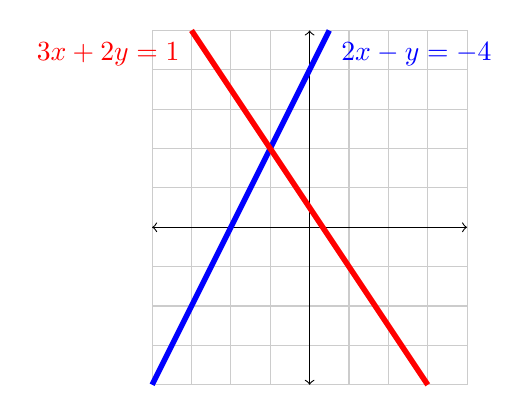
\begin{tikzpicture}[scale=.5]
\draw[thin,gray!40] (-4,-4) grid (4,5);
  \draw[<->] (-4,0)--(4,0);
  \draw[<->] (0,-4)--(0,5);

 \draw[line width=2pt,blue](-4, -4)--(0.5,5) node[below right]{$2x-y=-4$};
 \draw[line width=2pt,red](3, -4)--(-3,5) node[below left]{$3x+2y=1$};
\end{tikzpicture}
\end{image}

Given a system of two equations with two unknowns, there are three possible geometric outcomes.  First, the graphs of the two equations intersect at a point.  If this is the case, the system has exactly one solution. We say that the system is \dfn{consistent} and has a \dfn{unique solution}.  

\begin{image}[1.5in]
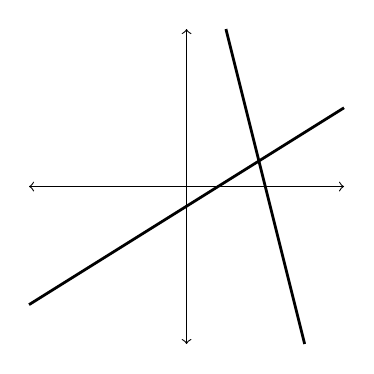
\begin{tikzpicture}[scale=.5]

  \draw[<->] (-4,0)--(4,0);
  \draw[<->] (0,-4)--(0,4);

 \draw[line width=1pt](-4, -3)--(4,2);
 \draw[line width=1pt](3, -4)--(1,4);
    
\end{tikzpicture}
\end{image}
Second, the two lines may have no points in common.  If this is the case, the system has no solutions.  We say that the system is \dfn{inconsistent}.  
\begin{image}[1.5in]
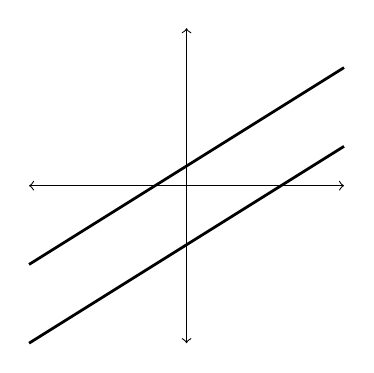
\begin{tikzpicture}[scale=.5]

  \draw[<->] (-4,0)--(4,0);
  \draw[<->] (0,-4)--(0,4);

 \draw[line width=1pt](-4, -4)--(4,1);
 \draw[line width=1pt](-4, -2)--(4,3);
    
\end{tikzpicture}
\end{image}
Finally, the two lines may coincide.  In this case, there are infinitely many points that satisfy both equations simultaneously.  We say that the system is consistent and has infinitely many solutions.
\begin{image}[1.5in]
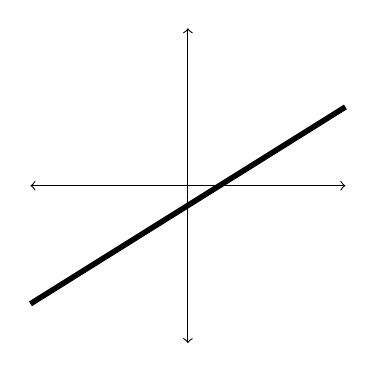
\begin{tikzpicture}[scale=.5]

  \draw[<->] (-4,0)--(4,0);
  \draw[<->] (0,-4)--(0,4);

 \draw[line width=2pt](-4, -3)--(4,2);
 
    
\end{tikzpicture}
\end{image}


\begin{example}\label{ex:systwoeqs2} Solve the system of equations and interpret your results geometrically.
$$\begin{array}{ccccc}
      -2x & +&y&= &3 \\
	 4x& -&2y&=&5
    \end{array}$$
\begin{explanation}
We will use elementary row operations.  Our goal is to eliminate $y$ from the first equation and eliminate $x$ from the second.  Observe that adding twice the first equation to the second equation accomplishes both tasks.
$$\begin{array}{ccccc}
      -2x & +&y&= &3 \\
	 0x& -&0y&=&11
    \end{array}$$
It is clear, however, that there are no values of $x$ and $y$ that would satisfy the second equation.  We conclude that the system is inconsistent.  Plotting the two lines in the same coordinate plane shows that the two lines are parallel.  
    \begin{image}[2in]
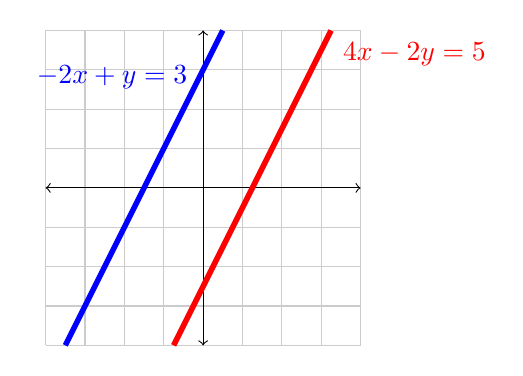
\begin{tikzpicture}[scale=.5]
\draw[thin,gray!40] (-4,-4) grid (4,4);
  \draw[<->] (-4,0)--(4,0);
  \draw[<->] (0,-4)--(0,4);

 \draw[line width=2pt,blue](-3.5, -4)--(0.5,4) node[below left=3mm]{$-2x+y=3$};
 \draw[line width=2pt,red](-0.75, -4)--(3.25,4) node[below right]{$4x-2y=5$};
    
\end{tikzpicture}
\end{image}
\end{explanation}
\end{example}

\begin{example} Solve the system of equations and interpret your results geometrically.
$$\begin{array}{ccccc}
      4x & +&3y&= &2 \\
	 x& +&\frac{3}{4}y&=&\frac{1}{2}
    \end{array}$$

\begin{explanation}
To eliminate $x$ from the second equation, we subtract one quarter of the first equation from the second.  This gives us

$$\begin{array}{ccccc}
      4x & +&3y&= &2 \\
	 0x& +&0y&=&0
    \end{array}$$
    
Unlike the situation in Example \ref{ex:systwoeqs2}, there are values of $x$ and $y$ that satisfy the second equation.  In fact, any ordered pair $(x, y)$ that satisfies the first equation will satisfy the second equation.  Thus, the solution set for this system is the same as the set of all solutions of $4x+3y=2$.  

When we plot the two equations of the original system, we find that the two lines coincide.


    \begin{image}[2.5in]
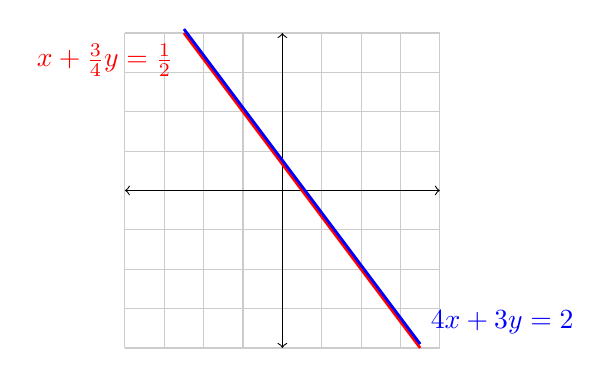
\begin{tikzpicture}[scale=.5]
\draw[thin,gray!40] (-4,-4) grid (4,4);
  \draw[<->] (-4,0)--(4,0);
  \draw[<->] (0,-4)--(0,4);  

 \draw[line width=1pt,red](-2.5, 4)node[below left]{$x +\frac{3}{4}y=\frac{1}{2}$}--(3.5,-4);
 \draw[line width=1pt,blue](-2.5, 4.1)--(3.5,-3.9) node[above right]{$4x+3y=2$};
 
    
\end{tikzpicture}
\end{image}
\end{explanation}
\end{example}

Given a linear system in two variables and more than two equations, we have a variety of geometric possibilities.  Three of them are depicted below.  First, it is possible for the graphs of all equations in the system to intersect at a single point, giving us a unique solution.  

\begin{image}[1.5in]
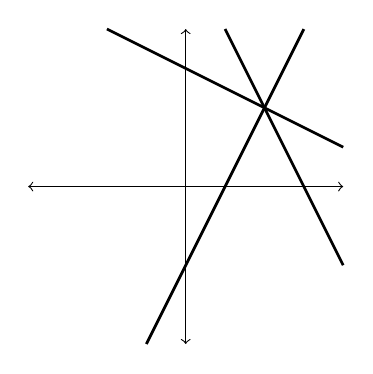
\begin{tikzpicture}[scale=.5]

  \draw[<->] (-4,0)--(4,0);
  \draw[<->] (0,-4)--(0,4);

 \draw[line width=1pt](-2, 4)--(4,1);
 \draw[line width=1pt](3, 4)--(-1,-4);
 \draw[line width=1pt](1, 4)--(4,-2);
    
\end{tikzpicture}
\end{image}

Second, it is possible for the graphs to have no points in common.

\begin{image}[3in]
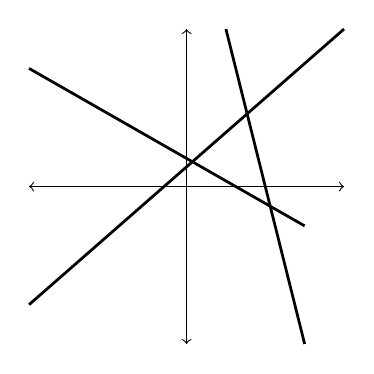
\begin{tikzpicture}[scale=.5]

  \draw[<->] (-4,0)--(4,0);
  \draw[<->] (0,-4)--(0,4);

 \draw[line width=1pt](-4, -3)--(4,4);
 \draw[line width=1pt](3, -4)--(1,4);
 \draw[line width=1pt](3, -1)--(-4,3);
    
\end{tikzpicture}\quad\quad
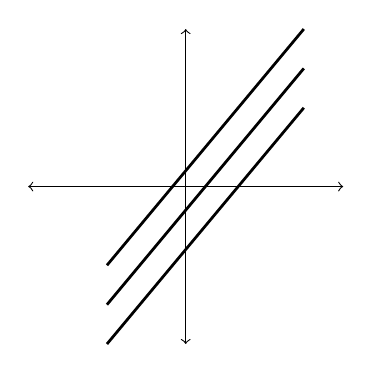
\begin{tikzpicture}[scale=.5]

  \draw[<->] (-4,0)--(4,0);
  \draw[<->] (0,-4)--(0,4);

 \draw[line width=1pt](-2, -3)--(3,3);
 \draw[line width=1pt](-2, -2)--(3,4);
 \draw[line width=1pt](-2, -4)--(3,2);
    
\end{tikzpicture}
\end{image}
If this is the case, the system is inconsistent.
\section*{Geometry of Linear Systems in Three Variables}
In Example \ref{ex:threeeqthreevars1} we solved the following linear system of three equations and three unknowns
$$\begin{array}{ccccccc}
      3x & -&y&+&z&= &0 \\
	 2x& +&y&+&2z&=&2\\
     x& +&4y&-&2z&=&11
    \end{array}$$
We found that the system has a unique solution $(1, 2, -1)$.  The graph of each equation is a plane.  The three planes intersect at a single point, as shown in the figure.
    
\begin{image}[2.5in]   
\tdplotsetmaincoords{70}{130}
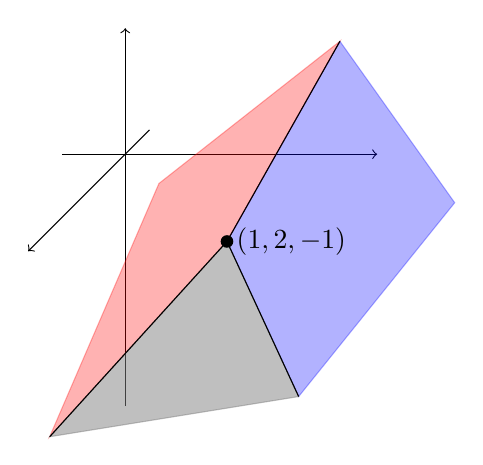
\begin{tikzpicture}[scale=0.8]
	\draw[->](-1,0,0)--(4,0,0) ;
    \draw[->](0,-4,0)--(0,2,0) ;
    \draw[->](0,0,-1)--(0,0,4) ;
    
   \filldraw[blue, opacity=0.3](2,-1,1)--(18/5,-3,11/5)--(6,0,2)--(47/13,2,7/13)--cycle;
   \filldraw[red, opacity=0.3] (2,-1,1)--(47/13,2,7/13)--(4,3,9)--(2/7,-3,27/7)--cycle;
   \filldraw[gray, opacity=0.5] (2,-1,1)--(2/7,-3,27/7)--(18/5,-3,11/5)--cycle;
     
     \draw[](2,-1,1)--(18/5,-3,11/5) ;
    \draw[](2,-1,1)--(47/13,2,7/13) ;
    \draw[](2,-1,1)--(2/7,-3,27/7) ;
    \fill[] (2,-1,1)node[right]{$(1,2,-1)$} circle (0.1cm);
    
\end{tikzpicture}
\end{image}


Given a linear system of three equations and three variables, there are three ways in which the system can be consistent.
First, the three planes could intersect at a single point, giving us a unique solution.
\begin{image}[1.5in]
\tdplotsetmaincoords{70}{130}
	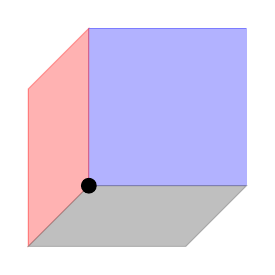
\begin{tikzpicture}
\filldraw[blue, opacity=0.3](0,0,0)--(2,0,0)--(2,2,0)--(0,2,0)--cycle;
\filldraw[red, opacity=0.3] (0,0,0)--(0,0,2)--(0,2,2)--(0,2,0)--cycle;
\filldraw[gray, opacity=0.5] (0,0,0)--(0,0,2)--(2,0,2)--(2,0,0)--cycle;
\fill[] (0,0,0) circle (0.1cm);
    \end{tikzpicture}
    \end{image}
    Second, the three planes can intersect in a line, forming a paddle-wheel shape.  In this case, every point along the line of intersection is a solution to the system, giving us infinitely many solutions.
    \begin{image}[2in]
\tdplotsetmaincoords{70}{130}
	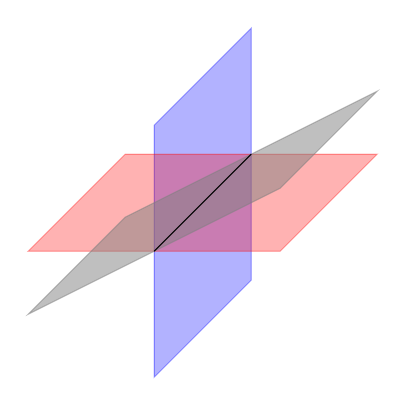
\begin{tikzpicture}[scale=0.8]
\filldraw[blue, opacity=0.3](0,-2,2)--(0,2,2)--(0,2,-2)--(0,-2,-2)--cycle;
\filldraw[red, opacity=0.3] (2,0,2)--(-2,0,2)--(-2,0,-2)--(2,0,-2)--cycle;
\filldraw[gray, opacity=0.5] (2,1,2)--(2,1,-2)--(-2,-1,-2)--(-2,-1,2)--cycle;
\draw[-](0,0,-2)--(0,0,2) ;
     \end{tikzpicture}
     \end{image}
     Finally, the three planes can coincide.  If this is the case, there are infinitely many solutions.
     \begin{image}[1.8in]
\tdplotsetmaincoords{70}{130}
	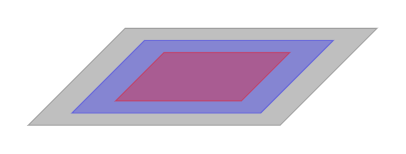
\begin{tikzpicture}[scale=0.8]
\filldraw[gray, opacity=0.5] (2,0,2)--(-2,0,2)--(-2,0,-2)--(2,0,-2)--cycle;
\filldraw[blue, opacity=0.3] (1.5,0,1.5)--(-1.5,0,1.5)--(-1.5,0,-1.5)--(1.5,0,-1.5)--cycle;
\filldraw[red, opacity=0.3] (1,0,1)--(-1,0,1)--(-1,0,-1)--(1,0,-1)--cycle;    	\end{tikzpicture}
\end{image}
There are four ways for a system to be inconsistent.  They are depicted below.
\begin{image}[4in]
\tdplotsetmaincoords{70}{130}
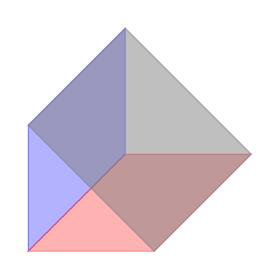
\begin{tikzpicture}[scale=0.8]
   \filldraw[blue, opacity=0.3](0,0,2)--(0,2,2)--(0,2,-2)--(0,0,-2)--cycle;
   \filldraw[red, opacity=0.3] (2,0,2)--(0,0,2)--(0,0,-2)--(2,0,-2)--cycle;
   \filldraw[gray, opacity=0.5] (0,2,2)--(0,2,-2)--(2,0,-2)--(2,0,2)--cycle;
\end{tikzpicture}\quad
	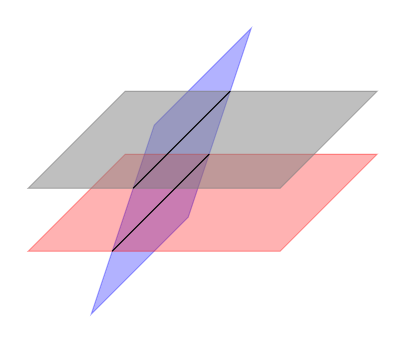
\begin{tikzpicture}[scale=0.8]
\filldraw[blue, opacity=0.3](-1,-1,2)--(0,2,2)--(0,2,-2)--(-1,-1,-2)--cycle;
\filldraw[red, opacity=0.3] (2,0,2)--(-2,0,2)--(-2,0,-2)--(2,0,-2)--cycle;
\filldraw[gray, opacity=0.5] (2,1,2)--(-2,1,2)--(-2,1,-2)--(2,1,-2)--cycle;
\draw[-](-2/3,0,-2)--(-2/3,0,2) ;
\draw[-](-1/3,1,-2)--(-1/3,1,2) ;
     \end{tikzpicture}
     
     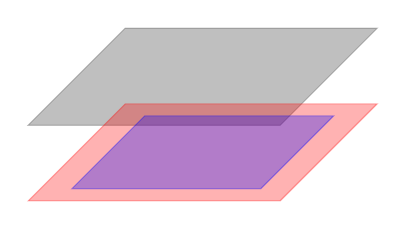
\begin{tikzpicture}[scale=0.8]
\filldraw[gray, opacity=0.5] (2,1.2,2)--(-2,1.2,2)--(-2,1.2,-2)--(2,1.2,-2)--cycle;
\filldraw[red, opacity=0.3] (2,0,2)--(-2,0,2)--(-2,0,-2)--(2,0,-2)--cycle;
\filldraw[blue, opacity=0.3] (-1.5,0,1.5)--(-1.5,0,-1.5)--(1.5,0,-1.5)--(1.5,0,1.5)--cycle;
	\end{tikzpicture}\quad
	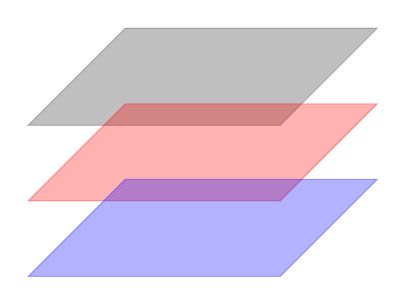
\begin{tikzpicture}[scale=0.8]
\filldraw[gray, opacity=0.5] (2,1.2,2)--(-2,1.2,2)--(-2,1.2,-2)--(2,1.2,-2)--cycle;
\filldraw[red, opacity=0.3] (2,0,2)--(-2,0,2)--(-2,0,-2)--(2,0,-2)--cycle;
\filldraw[blue, opacity=0.3] (2,-1.2,2)--(-2,-1.2,2)--(-2,-1.2,-2)--(2,-1.2,-2)--cycle;
	\end{tikzpicture}
    \end{image}     

\section*{Equivalent Systems and Elementary Row Operations}

In Exploration Problem \ref{init:systwoeqs1} we introduced elementary row operations and equivalent systems. We now make these definitions formal.

\begin{definition}[Elementary Row Operations]\label{def:elemrowops}
The following three operations performed on a linear system are called elementary row operations
\begin{enumerate}
\item\label{item:rowswap} Switching the order of two equations
\item\label{item:constantmult} Multiplying both sides of an equation by the same non-zero constant
\item\label{item:addrow} Adding a multiple of one equation to another
\end{enumerate}
\end{definition}

\begin{definition}\label{def:equivsystems} Two systems of linear equations are said to be equivalent if they have the same solution set.
\end{definition}

It is not difficult to see that performing a sequence of elementary row operations on a system of equations produces an equivalent system.  We can justify this by considering the row operations one at a time.  Clearly, the order of equations down does not affect the solution set, so \ref{item:rowswap} produces an equivalent system.  Next, you learned years ago that multiplying both sides of an equation by a non-zero constant does not change its solution set, which establishes that \ref{item:constantmult} produces an equivalent system.  It is also true that \ref{item:addrow} produces an equivalent system.  To see this, note that a multiple of an equation is still an equation, so if we add a multiple of an equation to another equation in the system, we are adding the same thing to both sides, which does not change the solution set of that equation, nor of the system.

% We would like to show that if a linear system $(A)$ is transformed into linear system $(B)$ through a sequence of elementary row operations then system $(A)$ is equivalent to system $(B)$.  We will illustrate this with a system of two equations and two unknowns.

% Consider the system
% \begin{equation}\label{eq:equivsystem1}
% \begin{array}{ccccc}
%       a_1x& +&b_1y&=&c_1\\
%       a_2x & +&b_2y&= &c_2 
%     \end{array}
%     \end{equation}
%     Suppose $(x', y')$ is a solution to this system.  
    
%     Let's switch the order of the two equations.
%     \begin{equation}\label{eq:equivsystem2}
% \begin{array}{ccccc}
%       a_2x & +&b_2y&= &c_2 \\
%       a_1x& +&b_1y&=&c_1
%     \end{array}
%     \end{equation}
% Clearly $(x', y')$ satisfies each equation in (\ref{eq:equivsystem2}) and is a solution to the system.  It is also clear that if $(x'',y'')$ is a solution to (\ref{eq:equivsystem2}), then $(x'', y'')$ is also a solution to (\ref{eq:equivsystem1}).  We conclude that systems (\ref{eq:equivsystem1}) and (\ref{eq:equivsystem2}) are equivalent.
    
%  If we multiply both sides of one equation (we'll pick the first one) by a non-zero constant $k$, we get
%  \begin{equation}\label{eq:equivsystem3}\begin{array}{ccccc}
%       ka_1x& +&kb_1y&=&kc_1\\
%       a_2x & +&b_2y&= &c_2 
%     \end{array}
%     \end{equation}
    
%     $$ka_1x'+kb_1y'=k(a_1x'+b_1y')=k(c_1)$$
%     So, $(x', y')$ satisfies (\ref{eq:equivsystem3}).  Now suppose $(x'', y'')$ satisfies (\ref{eq:equivsystem3}), then 
%     $$a_1x''+b_1y''=\frac{1}{k}(kc_1)=c_1$$
%     Therefore $(x'', y'')$ satisfies (\ref{eq:equivsystem1}).  Thus, systems (\ref{eq:equivsystem1}) and (\ref{eq:equivsystem3}) are equivalent.
    
%     Finally, let's add a multiple of the first row to the second row.
%     \begin{equation}\label{eq:equivsystem4}
% \begin{array}{cccccccccc}
%       a_1x& +&b_1y&&&&&=&c_1&\\
%       a_2x & +&b_2y&+&k(a_1x& +&b_1y)&= &c_2& +kc_1
%     \end{array}
%     \end{equation}
% We leave it as an exercise to show that systems (\ref{eq:equivsystem1}) and (\ref{eq:equivsystem4}) are equivalent.

%We will use $E_i$ to represent the left-hand side of the $i$th linear equation $a_{i1}x_1+a_{i2}x_2+\ldots +a_{in}x_n=b_i$ of a system.

%{\color{red}The following theorem and proof were adapted from Kuttler's text. systemsofequationsAlgebraicProceduresElementaryOperations.tex} \href{https://github.com/annadavismath/Kuttlers-Text/blob/6d9aa9e4e9fee0f8eff47d8c10405de89df12c4a/systemsofequationsAlgebraicProceduresElementaryOperations#L184}{Clickable Kuttler Ref.}

%\begin{theorem}[Elementary Operations and Solutions]\label{th:elementaryoperationsandsolns}
%Suppose a linear system includes equations:
%\begin{equation}
% \begin{array}{c}
 % E_i=b_i\\
 % E_j=b_j
%\end{array} \label{eq:system}
%\end{equation}
%Then the following systems have the same solution set as (\ref{eq:system}): 
%\begin{enumerate}
%\item\label{item:rowswap}   The original system with equations $i$ and $j$ switched.
%\begin{equation}
%	\begin{array}{c}
%	E_j=b_j\\
%	E_i=b_i
%	\end{array}
%	\label{eq:rowswap}
%	\end{equation}
%\item\label{item:constantmult}  The original system with equation $j$ replaced with a non-zero scalar multiple of $j$.
%\begin{equation}
%	\begin{array}{c}
%	E_i=b_i \\
%	kE_j=kb_j        
%	\end{array}
%	\label{eq:constantmult}
%\end{equation}
 % for any scalar $k$, provided $k\neq0$.
%\item\label{item:addmultrow} The original system with equation $j$ replaced with the sum of equation $j$ and a scalar multiple of equation $i$.
%\begin{equation}
 %     \begin{array}{c}
  %     E_i=b_i \\
   %    E_j+kE_i=b_j+kb_i
    %   \end{array}  
%	\label{eq:addmultrow}
%\end{equation}
%	for any scalar  $k$ (including $k=0$).
%\end{enumerate}
%\end{theorem}


%\begin{proof}[Proof of Property~\ref{item:rowswap}:] 
%We need to show that systems (\ref{eq:system}) and (\ref{eq:rowswap}) have the
%same solution set. 
%This is clear, because the system in (\ref{eq:rowswap}) is the original
%system, but listed in a different order. Changing the order does not
%affect the solution set. So if $( x_{1},\ldots ,x_{n})$ is a
%solution to one of (\ref{eq:system}) and (\ref{eq:rowswap}), then $( x_{1},\ldots ,x_{n}) $ is also a solution to the other.
%\end{proof}
%\begin{proof}[Proof of Property~\ref{item:constantmult}:] 
%Next we want to prove that systems (\ref{eq:system}) and (\ref{eq:constantmult}) have the
%same solution set. Let $( x_{1},\ldots ,x_{n})$ be a
%solution of $E_i=b_i,E_j=b_j,$. We want to show that it is a solution to $E_i=b_i,kE_j=kb_j$.
%Notice that the only difference between these two systems is that the second involves
%multiplying the equation, $E_j=b_j$ by the scalar $k$. Recall that when you multiply both sides of an 
%equation by the same number, the sides are still equal to each other. Hence if  $( x_{1},\ldots ,x_{n})$
%is a solution to $E_j=b_j$, then it will also be a solution to $kE_j=kb_j$. Hence, $( x_{1},\ldots ,x_{n})$ is also
%a solution to (\ref{eq:constantmult}). 

%Similarly, let $( x_{1},\ldots ,x_{n})$ be a solution of $E_i=b_i,kE_j=kb_j$. Then we can 
%multiply the equation $kE_j=kb_j$ by the scalar $1/k$, which is possible only because we have required that $k\neq
%0$. Just as above, this action preserves equality.
%Hence $( x_{1},\ldots ,x_{n})$ is also a solution to  $E_i=b_i,E_j=b_j.$ 
%\end{proof}
%\begin{proof}[Proof of Property~\ref{item:addmultrow}:]
%Finally, we will prove that the systems (\ref{eq:system}) and
%(\ref{eq:addmultrow}) have the same solution set. We will show that any
%solution of $E_i=b_i,E_j=b_j$ is also a solution of
%\ref{eq:addmultrow}. Then, we will show that any solution of \ref{eq:addmultrow}
%is also a solution of $E_i=b_i,E_j=b_j$.  Let $( x_{1},\ldots ,x_{n})$ be a solution to
%$E_i=b_i,E_j=b_j$. Then in particular it satisfies $E_i =
%b_i$. Hence, it satisfies the first equation in (\ref{eq:addmultrow}).
%Similarly, it also satisfies $E_j = b_j$. By our proof of
%(\ref{eq:constantmult}), it also satisfies $kE_i=kb_i$.  Notice that if we add
%$E_j$ and $kE_i$, the sum is equal to $b_j + kb_i$. Therefore, if
%$( x_{1},\ldots ,x_{n})$ satisfies $E_i=b_i,E_j=b_j$
%it must also satisfy $E_j+kE_i=b_j+kb_i$.

%Now suppose $( x_{1},\ldots ,x_{n})$  is a solution to the system 
%$E_i=b_i, E_j+kE_i=b_j+kb_i$. Then, in particular, it satisfies $E_i = b_i$. Again by our proof of (\ref{eq:constantmult}),
 %it is also a solution to $kE_i=kb_i$. Now if we subtract these equal quantities from both sides of 
%$E_j+kE_i=b_j+kb_i$ we obtain $E_j=b_j$, which shows that the solution also satisfies
%$E_i=b_i,E_j=b_j.$ 

%\end{proof}



\section*{Practice Problems}
\begin{problem}
Give a graphical illustration of each of the following scenarios for a system of three equations and two unknowns:
  \begin{enumerate}
  \item The system of three equations is inconsistent, but a combination of any two of the three equations forms a consistent system.
  \item The system is consistent and has a unique solution.
  \item The system is consistent and has infinitely many solutions.
  \item The system is inconsistent and no two equations form a consistent system.
  \end{enumerate}
\end{problem}

\begin{problem} 
Solve each system of linear equations or demonstrate that a solution does not exist, and interpret your results geometrically.
  \begin{problem}
  $$\begin{array}{ccccc}
      x & +&3y&= &4 \\
	 x& -&2y&=&-6
    \end{array}$$
    
    Solution: $$(\answer{-2},\answer{2})$$
  \end{problem}
  
  \begin{problem}
  $$\begin{array}{ccccc}
      -3x & +&2y&= &7 \\
	 6x& -&4y&=&5
    \end{array}$$
  \end{problem}
  
  
  \begin{problem}
$$\begin{array}{ccccccc}
      x & -&2y&+&z&= &0 \\
	 3x& -&2y&+&4z&=&2\\
     2x& -&y&+&2z&=&3
    \end{array}$$
    
Solution:    $$(\answer{4},\answer{1},\answer{-2})$$
\end{problem}
\end{problem}

  \begin{problem}
  Consider the following system of equations.
  $$\begin{array}{ccccc}
      kx & +&8y&= &4 \\
	 2x& +&ky&=&-2
    \end{array}$$
     \begin{problem}
Find all possible values of k such that this system has no solution.

Solution: $$k=\answer{4}$$
  \end{problem}
     \begin{problem}
Find all possible values of k such that this system has infinitely many solutions.

Solution: $$k=\answer{-4}$$
  \end{problem}
  \end{problem}

\begin{problem}
Why is there a non-zero provision in Part \ref{item:constantmult} of Definition \ref{def:elemrowops}?  Why is there not a non-zero provision in Part \ref{item:addrow}?
\end{problem}

\begin{problem}
Suppose the following system was obtained from system $(A)$ by adding twice the second row of $(A)$ to the first row.
$$\begin{array}{ccccc}
      8x &+ &3y&= &11\\
      3x&+ &2y&=&5      
    \end{array}$$
    Find system $(A)$.
    
    Answer:
    $$\begin{array}{ccccc}
      \answer{2}x &+ &\answer{-1}y&= &\answer{1}\\
      3x&+ &2y&=&5      
    \end{array}$$
    
\end{problem}

\begin{problem}
The following figures show a geometric depiction of two equivalent systems.  (The systems are equivalent because they have the same solution set.)  Can the first system be transformed into the second system by elementary row operations?  If so, how?

 \begin{image}[4in]
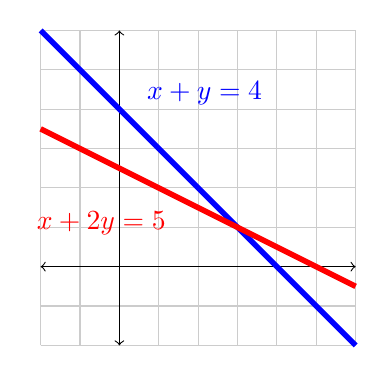
\begin{tikzpicture}[scale=.5]
\draw[thin,gray!40] (-2,-2) grid (6,6);
  \draw[<->] (-2,0)--(6,0);
  \draw[<->] (0,-2)--(0,6);

 \draw[line width=2pt,blue](-2, 6)node[below=8mm, right=12mm]{$x+y=4$}--(6,-2) ;
 \draw[line width=2pt,red](-2,3.5)node[below=12mm, right=-2mm]{$x+2y=5$}--(6,-0.5) ;
    
\end{tikzpicture}\quad\quad
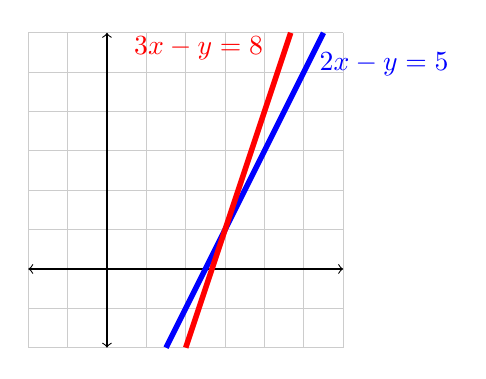
\begin{tikzpicture}[scale=.5]
\draw[thin,gray!40] (-2,-2) grid (6,6);
  \draw[<->] (-2,0)--(6,0);
  \draw[<->] (0,-2)--(0,6);

 \draw[line width=2pt,blue](1.5, -2)--(5.5,6) node[below=4mm, right=-2mm]{$2x-y=5$};
 \draw[line width=2pt,red](2, -2)--(14/3,6) node[below=2mm, left=2mm]{$3x-y=8$};
    
\end{tikzpicture}
\end{image}

\begin{hint}
Begin by carrying the first system to 
$$\begin{array}{ccccc}
      x & &&= &3\\
      & &y&=&1      
    \end{array}$$
    Then carry this system to the second system.
\end{hint}

\end{problem}

\begin{problem}
To demonstrate that system $(A)$ is equivalent to system $(B)$ we need to show the following:
\begin{center}
If $(x', y')$ is a solution of $(A)$, then $(x', y')$ is a solution of $(B)$.

and

If $(x'', y'')$ is a solution of $(B)$, then $(x'', y'')$ is a solution of $(A)$.
\end{center}

Show that  if system $(B)$ is obtained from system $(A)$ using elementary row operation \ref{item:constantmult} or elementary row operation \ref{item:addrow}, then $(B)$ and $(A)$ are equivalent.
\end{problem}
% \begin{problem}
% Demonstrate that elementary row operations are reversible by answering the following questions.  Be specific about the elementary row operation that you would use.
% \begin{enumerate}
% \item We obtained system (\ref{eq:equivsystem2}) from system (\ref{eq:equivsystem1}) by swapping the two equations. How would we obtain system (\ref{eq:equivsystem1}) from system (\ref{eq:equivsystem2})?
% \item We obtained system (\ref{eq:equivsystem3}) from system (\ref{eq:equivsystem1}) by multiplying one of the equations by a non-zero constant $k$.  How would we obtain system (\ref{eq:equivsystem1}) from system (\ref{eq:equivsystem3})?
% \item We obtained system (\ref{eq:equivsystem4}) from system (\ref{eq:equivsystem1}) by adding a multiple of one of the equations to the other.  How would we obtain system (\ref{eq:equivsystem1}) from system (\ref{eq:equivsystem4})?
% \end{enumerate}
% \end{problem}

\end{document} 
